% !TEX program = xelatex
\documentclass[10pt,fontset=none,twocolumn]{ctexart}
\usepackage[a4paper,top=1.8cm,bottom=1.8cm,left=1.5cm,right=1.5cm]{geometry}
\usepackage{fontspec}
\usepackage{xeCJK}
\IfFontExistsTF{SimSun}{\setCJKmainfont[BoldFont=SimHei,ItalicFont=SimSun]{SimSun}}{\setCJKmainfont{FandolSong-Regular}}
\IfFontExistsTF{SimHei}{\setCJKsansfont{SimHei}}{\setCJKsansfont{FandolHei-Regular}}
\usepackage{amsmath,amssymb,bm}
\usepackage{cite}
\usepackage{booktabs}
\usepackage{array}
\usepackage{graphicx}
\usepackage{url}
\usepackage{enumitem}

\setlength{\parskip}{0pt}
\setlength{\parindent}{2em}
\setlist[enumerate]{leftmargin=1.4em,itemsep=0pt,topsep=2pt}

\newcommand{\gsid}{\mathrm{GeoSemID}}
\newcommand{\Experts}{\mathcal{M}}
\newcommand{\POIs}{\mathcal{P}}
\newcommand{\Users}{\mathcal{U}}
\newcommand{\Train}{\mathcal{D}_{\mathrm{tr}}}
\newcommand{\HitTrain}{\mathcal{D}_{\mathrm{hit}}}
\newcommand{\Ind}{\mathbb{I}}

\title{\bfseries 面向下一兴趣点预测的受约束地理语义标识与效用监督动态多专家检索}
\author{匿名作者}
\date{}

\begin{document}
\maketitle

\begin{abstract}
下一兴趣点（POI）预测需要从大规模、异构的位置目录中识别用户下一次最可能访问的地点。现有方法通常将 POI 表示为彼此孤立的标识符，并依赖单一召回信号，因此在稀疏轨迹和长尾地点上容易出现候选漏召回。本文提出 GeoSemID 框架，将受约束的地理语义标识与效用监督的动态多专家检索结合。GeoSemID 为每个 POI 构造粗粒度地理编码、细粒度地理编码、规范化类别编码，以及由 POI 元数据离线生成并验证的语义编码。空间、转移、时间和语义专家产生互补候选；其中基于计数的专家采用可靠性感知的层级回退，空间与语义专家采用同尺度的显式证据融合。路由器仅利用至少一个专家已召回真实目标的训练样本进行监督，并融合基于排序百分位的证据。随后，候选约束语言模型仅对合法候选 POI 标识计算条件似然，实现候选覆盖与条件排序的分离。在 CA、NYC 和 TKY 的 1,818、988 和 2,206 个测试样本上，GeoSemID 的 HR@10 分别达到 42.48\%、44.65\% 和 46.85\%，动态融合的 Top-50 候选召回率分别达到 60.00\%、62.40\% 和 64.20\%。
\end{abstract}

\noindent\textbf{关键词：} 下一兴趣点预测；地理语义标识；多专家检索；动态路由；大语言模型

\section{引言}
\label{sec:introduction}

下一兴趣点（POI）预测是智能交通系统、基于位置的服务和个性化出行辅助中的一个基础问题。一个实用的预测器必须在平衡用户长期稳定偏好与即时移动意图的同时，考虑时间规律性、地理可达性以及位置的功能语义。尽管序列和时空模型已显著提升了轨迹编码能力，但其决策空间仍然是一个由海量异构 POI 构成的庞大目录。

原子的 POI 标识符（ID）虽然提供了精确的区分度，但由于缺乏可复用的结构关系，在稀疏位置上面临严重的泛化瓶颈。一个长尾 POI 即使在地理上邻近、功能上相似，或在上下文用法上可比于一个高频 POI，这些潜在关系也无法在仅依赖 ID 的模型中自动流转。虽然元数据和连续向量表征（embeddings）提供了重要信号并构成强基线，但它们本身并不能为地理、类别 and 上下文关联定义出离散且可复用的层级，以在统计稀疏时进行回退平滑。

因此，候选集生成阶段（检索阶段）不仅仅是一个简单的预处理步骤。空间、转移、时间和语义信号捕捉了不同的移动约束，且不同轨迹样本中这些信号的有效性是存在差异的。单一检索器或全局固定的融合规则极易遗漏真实目标；一旦目标未被召回至候选集中，后续的重排器将彻底失去预测正确的可能性。当使用大语言模型（LLM）来推理异构轨迹上下文、但最终必须从庞大的离散 POI 目录中进行选择时，这一问题尤为突出。

针对上述挑战，我们提出 GeoSemID，一个将结构化 POI 表征与样本级候选生成相结合的检索增强预测框架。GeoSemID 为每个原子 POI ID 补充了受约束的地理、类别和语义编码。空间、转移、时间和语义专家各自检索出互补的候选列表；一个受效用监督的路由器在样本级别学习专家的即时可靠性，并通过名次百分位融合使各专家分值具备可比性。最终，动态融合的专家检索证据被显式保留并输入给候选约束的 LLM 重排器，而不是在检索后被直接丢弃。

本文的主要贡献包括三个方面：
\begin{itemize}
\item 我们引入了 GeoSemID 编码表示，在保留原子 POI 唯一性的同时，为稀疏和长尾地点提供可复用的地理、类别与语义层级结构。
\item 我们设计了效用监督的动态多专家检索机制，利用训练样本的真实目标名次定义样本级专家效用，并引导名次可比的候选集动态融合。
\item 我们构建了感知检索证据的候选约束重排协议，实现了候选集召回覆盖与条件选择性排序的阶段性解耦，并在解码时避免了发散的 POI-ID 生成。
\end{itemize}

\section{相关工作}
\label{sec:related_work}

\subsection{时空建模与语义兴趣点表示}
\label{subsec:rw_representation}

早期的序列推荐模型（如分解个性化马尔可夫链 FPMC）主要建模先前选择与后续选择之间的依赖关系 \cite{rendle2010}。在移动出行领域，ST-RNN \cite{liu2016} 显式地将空间和时间上下文引入到循环预测中，而基于注意力的轨迹编码器（如 DeepMove \cite{feng2018}）提升了对历史移动规律的建模能力。近年来，包括 GETNext \cite{yang2022} 在内的流感知时空注意力模型进一步建模了非局部的时空相关性。这些工作极大提升了轨迹编码的精度，但强轨迹编码器本身并不能解决候选 POI 之间的地理、功能和语义关联如何表达与共享的问题。

大量代表性方法仍然主要依赖原子 POI ID、类别特征、经纬度坐标或其简单的浅层组合。虽然连续语义向量（embeddings）能有效表达位置相似度，但离散标识符（identifiers）能额外提供可复用的符号化结构。GeoSemID 旨在补充而非替代原子 ID 表达：它使得地理、类别和受约束的语义编码能够在检索、回退平滑以及重排阶段同时生效。这种定位并不否认现有向量表征的强大，而是针对统计稀疏场景下对显式、可复用层级结构的特定需求。

\subsection{兴趣点推荐中的候选检索与大模型重排}
\label{subsec:rw_retrieval_ranking}

庞大的 POI 目录促成了“先检索、后重排”的两阶段推荐流水线，因为候选生成直接决定了下游重排器的决策上限。地理邻近性、转移概率、时间偏好和向量相似度提供了互补的检索源，然而，简单的并集或全局固定的权重融合无法表达“常规通勤”与“探索性拜访”对不同检索证据的即时依赖。原先的 CoMaPOI 框架证明了在面向大模型的 POI 推荐中，将轨迹理解、候选集筛选和最终预测进行解耦的系统价值 \cite{zhong2025}。

基于 LLM 的 POI 系统能够将长期画像、近期轨迹、时间以及位置元数据序列化到统一的文本接口中，但它们仍面临庞大的离散输出空间以及候选顺序/上下文长度等负面效应。候选约束的似然得分计算比起无约束的自由生成更加可控。然而，下游重排接口通常无法显式地保留检索阶段的置信度来源。GeoSemID 针对性地在轨迹样本层面学习专家的实时效用，在统一的尺度上融合多专家排名，并将候选集的检索证据直接传递给最终的约束重排器。这种设计将检索可靠性与重排区分度视为相互耦合的两个阶段。

\section{问题定义}
\label{sec:problem}

\subsection{下一兴趣点预测}

设用户集合和 POI 集合分别为 $\Users=\{u_1,\ldots,u_{|\Users|}\}$ 和 $\POIs=\{p_1,\ldots,p_{|\POIs|}\}$。每个 POI $p$ 拥有对应的元数据
\begin{equation}
\bm{m}_{p}
=
\langle n_p,c_p,\bm{g}_p,\bm{a}_p\rangle,
\label{eq:poi_metadata}
\end{equation}
其中 $n_p$ 是 POI 名称，$c_p$ 是其功能类别，$\bm{g}_p$ 包含经纬度坐标及行政区划信息，$\bm{a}_p$ 记录其他补充属性。

用户 $u$ 在序列位置 $i$ 的签到记录表示为
\begin{equation}
x_{u,i}=\langle p_{u,i},t_{u,i}\rangle.
\label{eq:checkin}
\end{equation}
当预测目标为 $p_u^{*}=p_{u,n_u}$ 时，可观测轨迹为 $\{x_{u,1},\ldots,x_{u,n_u-1}\}$。给定近期窗口长度 $L$，轨迹被划分为：
\begin{align}
\mathcal{T}_{u}^{H}
&=
\{x_{u,1},\ldots,x_{u,n_u-L-1}\},
\label{eq:historical_trajectory}\\
\mathcal{T}_{u}^{C}
&=
\{x_{u,n_u-L},\ldots,x_{u,n_u-1}\},
\label{eq:current_trajectory}
\end{align}
其中 $\mathcal{T}_{u}^{H}$ 刻画长期移动偏好，$\mathcal{T}_{u}^{C}$ 描述即时移动上下文。

由于完整 POI 目录包含大量无关项，我们将下一兴趣点预测定义为两个耦合的任务：首先，检索模型构建一个紧凑的候选集 $\mathcal{C}_u\subset\POIs$ 并最大化其召回覆盖率：
\begin{equation}
\Pr(p_u^{*}\in\mathcal{C}_u
\mid
\mathcal{T}_{u}^{H},\mathcal{T}_{u}^{C},\{\bm{m}_p\}_{p\in\POIs}).
\label{eq:coverage_objective}
\end{equation}
接着，重排器预测最终地点：
\begin{equation}
\widehat{p}_{u}
=
\arg\max_{p\in\mathcal{C}_u}
P_{\psi}
\left(
p\mid
\mathcal{T}_{u}^{H},
\mathcal{T}_{u}^{C},
\mathcal{C}_u,
\gsid(p),
\bm{\xi}_{u,p}
\right),
\label{eq:final_prediction}
\end{equation}
其中 $\gsid(p)$ 为候选 POI $p$ 的结构化地理语义标识，$\bm{\xi}_{u,p}$ 记录其对应的专家检索证据。若真实目标 $p_u^{*}\notin\mathcal{C}_u$，端到端预测必然失败；因此候选覆盖与条件排序质量需独立评估。

\subsection{受约束地理语义标识}

为了使 POI 之间共享地理、功能与上下文语义，定义
\begin{equation}
\gsid(p)
=
[
z_{p}^{\mathrm{cg}},
z_{p}^{\mathrm{fg}},
z_{p}^{\mathrm{cat}},
z_{p}^{\mathrm{sem}}
],
\label{eq:geosemid_definition}
\end{equation}
其中 $z_{p}^{\mathrm{cg}}$ 与 $z_{p}^{\mathrm{fg}}$ 代表粗、细粒度地理网格编码，$z_{p}^{\mathrm{cat}}$ 代表规范化的功能类别编码，$z_{p}^{\mathrm{sem}}$ 代表受约束的语义编码。

前三个编码通过元数据确定性生成：
\begin{align}
z_{p}^{\mathrm{cg}}&=\rho_{\mathrm{cg}}(\bm{g}_p),&
z_{p}^{\mathrm{fg}}&=\rho_{\mathrm{fg}}(\bm{g}_p),&
z_{p}^{\mathrm{cat}}&=\rho_{\mathrm{cat}}(c_p).
\label{eq:deterministic_codes}
\end{align}
语义编码由微调的大模型离线单次映射生成，并通过固定语法验证：
\begin{equation}
z_{p}^{\mathrm{sem}}
=
\operatorname{Validate}
\left[
G_{\phi}\!\left(\mathcal{I}(\bm{m}_p)\right)
\right],
\label{eq:semantic_generation}
\end{equation}
其中 $\mathcal{I}(\cdot)$ 表示元数据序列化提示词，$G_{\phi}$ 是生成器，$\operatorname{Validate}(\cdot)$ 强制执行预设语法。该生成器仅执行单次从元数据到编码的映射，而非自治 Agent。

语义编码的目标形式固定为：
\begin{equation}
y_p^{\mathrm{sem}}
=
\langle
y_p^{\mathrm{intent}},
y_p^{\mathrm{attribute}},
y_p^{\mathrm{context}}
\rangle
\in
\mathcal{V}_{i}\times\mathcal{V}_{a}\times\mathcal{V}_{c},
\label{eq:semantic_schema}
\end{equation}
其中不包含类别字段，类别由 $z_p^{\mathrm{cat}}$ 唯一表达。语义标签表示访问意图、区别性服务属性和上下文用法。解码在贪心搜索下如果无效会重生成一次，若二次仍非法则映射为 \texttt{UNK} 并统计无效率。

\subsection{上下文自适应多专家检索}

令 $\Experts=\{\mathrm{sp},\mathrm{tr},\mathrm{tp},\mathrm{se}\}$ 表示空间、转移、时间和语义检索专家。在离线训练阶段，每个专家对全量目录评分，在在线推理阶段各自返回 top-$K_0$ 候选列表：
\begin{equation}
\mathcal{C}_{u}^{(m)}
=
\operatorname{TopK}_{K_0}
\{r_{u}^{(m)}(p):p\in\POIs\}.
\label{eq:expert_candidate}
\end{equation}
样本级路由器从可观测轨迹上下文估计专家分配权重 $\bm{\pi}_u=\{\pi_u^{(m)}\}_{m\in\Experts}$，并融合名次归一化的专家证据产生最终的 $\mathcal{C}_u$。训练集的真实目标名次仅在训练阶段用于构造路由监督，在验证和测试时绝对不可见。

\section{方法论}
\label{sec:method}

\subsection{框架概述}

GeoSemID 包含三个耦合阶段：首先，离线将 POI 元数据映射为包含 HSID 的层级编码，保留原始 ID 作为精确区分；其次，转移和时间检索器利用可靠性感知层级回退，空间和语义检索器计算物理/语义层级证据，路由器根据效用软标签进行样本级动态路由融合；最后，候选约束的 LLM 在保留专家证据的上下文中，显式计算候选 POI 标识的条件概率名次。

该框架的创新边界并非“使用 Qwen”或简单堆砌四个专家，而是：（i）受约束且可复用的地理语义编码，为稀疏 POI 提供结构化层级回退；（ii）针对动态路由器的样本级效用监督而非静态加权；（iii）检索置信度证据到下游重排的端到端保留。

\subsection{离线 GeoSemID 编码构建}
\label{subsec:geosemid}

\subsubsection{语义编码监督与数据隔离}

语义生成器基于以下数据集训练：
\begin{equation}
\mathcal{D}_{\mathrm{sem}} = \{ (\mathcal{I}(\bm{m}_p),y_p^{\mathrm{sem}}) \},
\label{eq:semantic_dataset}
\end{equation}
采用 Token 级别的负对数似然损失：
\begin{equation}
\mathcal{L}_{\mathrm{sem}}
=
-
\sum_{(\bm{x},\bm{y})\in\mathcal{D}_{\mathrm{sem}}}
\sum_{\ell=1}^{|\bm{y}|}
\log P_{\phi}(y_{\ell}\mid\bm{x},y_{<\ell}).
\label{eq:semantic_loss}
\end{equation}
目标序列化格式固定为如
\begin{equation}
\texttt{<INTENT=i;ATTRIBUTE=a;CONTEXT=c>},
\label{eq:serialization_example}
\end{equation}
解码仅接受对应词表内的值。为防止轨迹标签泄露，生成器 $G_{\phi}$ 仅接收 POI 自身的元数据，而不接收用户 ID、历史 check-in 序列或评估集标签。在标准转导评估中，目录的元数据可离线批量生成，但专家检索用到的签到转移统计量必须严格局限于训练集。

\subsubsection{检索特征表征}

实现中将结构化标识与 POI 元数据序列化后交给检索编码器：
\begin{equation}
\bm{e}_{p}^{\mathrm{gs}}
=
\operatorname{Enc}_{\mathrm{ret}}
\left(
\operatorname{Serialize}
\left[
\gsid(p),\bm{m}_p
\right]
\right).
\label{eq:geosemid_embedding}
\end{equation}
该序列化保留了规范化的 POI ID 以提供精细刻画，同时将 GeoSemID 各字段暴露给同一检索编码器。这适用于本地和 API 的嵌入模型，无需训练独立的标识嵌入表或投影层。

\subsection{基于计数统计的可靠性感知层级回退}
\label{subsec:backoff}

转移和时间专家依赖有限的签到转移次数。对于计数专家 $m\in\{\mathrm{tr},\mathrm{tp}\}$，设精确概率为 $P_{u,\mathrm{ex}}^{(m)}(p)$，第 $l$ 层标识引导的概率为 $P_{u,l}^{(m)}(p)$。精确概率的样本量支持度为 $N_u^{(m)}$，其可靠性系数定义为：
\begin{equation}
\lambda_{u}^{(m)}
=
\frac{N_{u}^{(m)}}{N_{u}^{(m)}+\alpha_m},
\label{eq:reliability}
\end{equation}
其中 $\alpha_m>0$ 为平滑常数。两项概率在对数空间前进行线性插值：
\begin{align}
P_u^{(m)}(p)
={}&
\lambda_u^{(m)}P_{u,\mathrm{ex}}^{(m)}(p)
\nonumber\\
&+
(1-\lambda_u^{(m)})
\sum_{l\in\mathcal{L}_m}
\omega_l^{(m)}P_{u,l}^{(m)}(p),
\label{eq:unified_backoff_probability}\\
r_u^{(m)}(p)
={}&
\log\!\left(P_u^{(m)}(p)+\epsilon\right),
\label{eq:unified_backoff}
\end{align}
其中 $\epsilon>0$ 为防零溢出小值，$\sum_l\omega_l^{(m)}=1$。对于给定标识值 $z$，其 POI 桶的大小为：
\begin{equation}
\nu_l(z)
=
\left|\{p'\in\POIs:z_{p'}^{(l)}=z\}\right|.
\label{eq:identifier_bucket_size}
\end{equation}
将层级类别概率除以 $\nu_l(z)$ 可以将粗粒度概率平摊到具体 POI 上，避免桶内 POI 概率虚高。对于概率项，使用加性平滑：
\begin{equation}
P_{\delta}(b\mid a)
=
\frac{N(a,b)+\delta}{N(a)+\delta|\mathcal{Y}|},
\label{eq:additive_smoothing}
\end{equation}
其中 $\mathcal{Y}$ 是可能的结果词表。

\subsection{专用检索专家}
\label{subsec:experts}

\subsubsection{空间专家}

设 $\bm{g}_{u}^{\mathrm{last}}$ 为轨迹最后坐标，$\bm{g}_{u}^{\mathrm{ctr}}$ 为中位数中心。基于大圆距离的分数映射到 $[0,1]$ 为：
\begin{equation}
\begin{aligned}
s_{u,\mathrm{dist}}^{(\mathrm{sp})}(p)
={}&\frac{1}{2}\exp\!\left(-\widetilde d_{\mathrm{hav}}
(\bm{g}_{u}^{\mathrm{last}},\bm{g}_{p})\right)\\
&+\frac{1}{2}\exp\!\left(-\widetilde d_{\mathrm{hav}}
(\bm{g}_{u}^{\mathrm{ctr}},\bm{g}_{p})\right),
\end{aligned}
\label{eq:spatial_exact}
\end{equation}
其中 $\widetilde d_{\mathrm{hav}}$ 是除以训练集中位数距离后的哈弗辛距离。区域层级指示函数为：
\begin{align}
b_{u,\mathrm{cg}}^{(\mathrm{sp})}(p)
&=
\Ind[z_p^{\mathrm{cg}}\in\mathcal{R}_{u}^{\mathrm{cg}}],
&
b_{u,\mathrm{fg}}^{(\mathrm{sp})}(p)
&=
\Ind[z_p^{\mathrm{fg}}\in\mathcal{R}_{u}^{\mathrm{fg}}],
\label{eq:spatial_backoff}
\end{align}
空间专家得分融合同尺度的距离和区域证据：
\begin{equation}
r_u^{(\mathrm{sp})}(p)
=
\zeta_{\mathrm{sp}}s_{u,\mathrm{dist}}^{(\mathrm{sp})}(p)
+
(1-\zeta_{\mathrm{sp}})
\sum_{l\in\{\mathrm{cg},\mathrm{fg}\}}
\omega_l^{(\mathrm{sp})}b_{u,l}^{(\mathrm{sp})}(p).
\label{eq:spatial_fusion}
\end{equation}
其中 $\zeta_{\mathrm{sp}}\in[0,1]$ 且 $\omega_l^{(\mathrm{sp})}$ 在验证集上选定。

\subsubsection{转移专家}

设 $p_u^{\mathrm{last}}$ 为最后签到。精确概率与层级回退概率为：
\begin{equation}
P_{u,\mathrm{ex}}^{(\mathrm{tr})}(p)
=
P_{\delta_{\mathrm{tr}}}(p\mid p_u^{\mathrm{last}}).
\label{eq:transition_exact}
\end{equation}
对于 $l\in\{\mathrm{fg},\mathrm{cat},\mathrm{sem}\}$，
\begin{equation}
P_{u,l}^{(\mathrm{tr})}(p)
=
\frac{
P_{\delta_{\mathrm{tr}},l}
(z_p^{(l)}\mid z_{p_u^{\mathrm{last}}}^{(l)})
}{
\nu_l(z_p^{(l)})
}.
\label{eq:transition_backoff}
\end{equation}
支持度 $N_u^{(\mathrm{tr})}$ 为训练集里从 $p_u^{\mathrm{last}}$ 触发的转移频次。

\subsubsection{时间专家}

设 $\tau_u$ 为当前时间分桶。精确概率与回退层级为：
\begin{equation}
P_{u,\mathrm{ex}}^{(\mathrm{tp})}(p)
=
P_{\delta_{\mathrm{tp}}}(p\mid u,\tau_u).
\label{eq:temporal_exact}
\end{equation}
\begin{equation}
P_{u,l}^{(\mathrm{tp})}(p)
=
\frac{P_{\delta_{\mathrm{tp}},l}(z_p^{(l)}\mid\tau_u)}
{\nu_l(z_p^{(l)})},
\quad
l\in\{\mathrm{cat},\mathrm{sem}\}.
\label{eq:temporal_backoff}
\end{equation}
支持度 $N_u^{(\mathrm{tp})}$ 为用户 $u$ 在时间桶 $\tau_u$ 里的签到数。

\subsubsection{语义专家}

从序列化历史及当前轨迹中生成意图检索向量：
\begin{equation}
\bm{q}_{u}^{\mathrm{sem}}
=
\operatorname{Enc}_{\mathrm{ret}}
\left(
\operatorname{Serialize}
\left[\mathcal{T}_{u}^{H},\mathcal{T}_{u}^{C}\right]
\right).
\label{eq:semantic_query}
\end{equation}
语义余弦相似度归一化为 $[0,1]$：
\begin{equation}
s_{u,\mathrm{sim}}^{(\mathrm{se})}(p)
=
\frac{1+\operatorname{cos}\!\left(
\bm{q}_{u}^{\mathrm{sem}},\bm{e}_{p}^{\mathrm{gs}}
\right)}{2},
\label{eq:semantic_exact}
\end{equation}
其 GeoSemID 重合证据为：
\begin{equation}
\begin{aligned}
b_{u,l}^{(\mathrm{se})}(p)
&=
\frac{1}{|\mathcal{T}_{u}^{C}|}
\sum_{x_{u,i}\in\mathcal{T}_{u}^{C}}
\Ind[z_{p_{u,i}}^{(l)}=z_p^{(l)}],\\
&\hspace{1.2em}
 l\in\{\mathrm{cg},\mathrm{fg},\mathrm{cat},\mathrm{sem}\}.
\end{aligned}
\label{eq:semantic_backoff}
\end{equation}
语义得分融合公式为：
\begin{equation}
r_u^{(\mathrm{se})}(p)
=
\zeta_{\mathrm{se}}s_{u,\mathrm{sim}}^{(\mathrm{se})}(p)
+
(1-\zeta_{\mathrm{se}})
\sum_{l\in\{\mathrm{cg},\mathrm{fg},\mathrm{cat},\mathrm{sem}\}}
\omega_l^{(\mathrm{se})}b_{u,l}^{(\mathrm{se})}(p).
\label{eq:semantic_fusion}
\end{equation}

\subsection{效用监督样本级路由器}
\label{subsec:router}

\subsubsection{可观测路由上下文}

路由器输入不含目标信息，其特征向量定义为：
\begin{equation}
\bm{q}_{u}
=
[
\bm{h}_{u}^{H}
\Vert
\bm{h}_{u}^{C}
\Vert
\bm{e}_{\tau_u}
\Vert
\bm{s}_{u}^{\mathrm{mob}}
\Vert
\bm{s}_{u}^{\mathrm{gs}}
],
\label{eq:routing_context}
\end{equation}
包含轨迹表示、时间编码、移动性指标（移动距离、回转半径等）以及 GeoSemID 转移统计量。路由器预测输出：
\begin{equation}
\bm{\pi}_{u}
=
\operatorname{softmax}(f_{\theta}(\bm{q}_{u})/T_r).
\label{eq:router_output}
\end{equation}

\subsubsection{训练特有效用监督}

仅在训练期间，设真实目标 $p_u^*$ 被召回时的名次为 $\operatorname{rank}_u^{(m)}(p_u^*)$，专家 $m$ 的效用为：
\begin{equation}
a_{u}^{(m)}
=
\begin{cases}
1-\dfrac{\operatorname{rank}_{u}^{(m)}(p_u^{*})-1}{K_0},
&p_u^{*}\in\mathcal{C}_{u}^{(m)},\\[7pt]
0,&p_u^{*}\notin\mathcal{C}_{u}^{(m)},
\end{cases}
\label{eq:expert_utility}
\end{equation}
效用软目标为：
\begin{equation}
q_{u}^{(m)}
=
\frac{
\Ind[a_u^{(m)}>0]\exp(a_{u}^{(m)}/\tau_q)
}{
\sum_{j\in\Experts}
\Ind[a_u^{(j)}>0]\exp(a_{u}^{(j)}/\tau_q)
}.
\label{eq:utility_target}
\end{equation}
训练集 $\mathcal{D}_{\mathrm{router}}$ 仅包含至少被一个专家召回的样本：
\begin{equation}
\mathcal{D}_{\mathrm{router}}
=
\{u\in\Train:\max_{m\in\Experts}a_u^{(m)}>0\}.
\label{eq:router_training_set}
\end{equation}
路由器的优化损失函数为：
\begin{equation}
\mathcal{L}_{\mathrm{router}}
=
-
\sum_{u\in\mathcal{D}_{\mathrm{router}}}
\sum_{m\in\Experts}
q_{u}^{(m)}\log\pi_{u}^{(m)}.
\label{eq:router_loss}
\end{equation}

\subsection{名次可比动态融合与证据保留}
\label{subsec:fusion}

由于分数尺度不同，专家分数不直接累加，而是转化为列表百分位名次：
\begin{equation}
\overline r_{u}^{(m)}(p)
=
\begin{cases}
1-\dfrac{\operatorname{rank}_{u}^{(m)}(p)-1}{K_0},
&
p\in\mathcal{C}_{u}^{(m)},\\[7pt]
0,
&
p\notin\mathcal{C}_{u}^{(m)}.
\end{cases}
\label{eq:rank_percentile}
\end{equation}
并集候选池和动态融合评分为：
\begin{align}
\widetilde{\mathcal{C}}_u
&=
\bigcup_{m\in\Experts}\mathcal{C}_{u}^{(m)},
\label{eq:union_pool}\\
s_u(p)
&=
\sum_{m\in\Experts}
\pi_u^{(m)}\overline r_u^{(m)}(p).
\label{eq:dynamic_fusion}
\end{align}
最终候选集为
\begin{equation}
\mathcal{C}_u
=
\operatorname{TopK}_{K}
\{s_u(p):p\in\widetilde{\mathcal{C}}_u\}.
\label{eq:final_candidate}
\end{equation}
对于保留下来的候选，其携带的检索证据向量为：
\begin{equation}
\bm{\xi}_{u,p}
=
\mathop{\Vert}_{m\in\Experts}
[
\pi_u^{(m)},
\overline r_u^{(m)}(p),
\Ind[p\in\mathcal{C}_u^{(m)}]
].
\label{eq:evidence_vector}
\end{equation}

\subsection{可复现的候选约束大模型重排}
\label{subsec:ranker}

\subsubsection{结构化提示词}

每个 Prompt 包含五个固定字段：\texttt{HISTORY\_PROFILE}、\texttt{CURRENT\_TRAJECTORY}、\texttt{PREDICTION\_TIME}、\texttt{CANDIDATES}（带编码及证据）以及 \texttt{OUTPUT}（目标候选 ID）。为消除位置偏差，训练时候选记录随机置换，推理时按 canonical ID 进行字母序重排。若输入超出限制，则先截断老旧历史。

\subsubsection{显式候选概率似然}

令 $\operatorname{tok}(p)$ 表示候选 canonical ID 的 tokenizer 编码。模型不用自由解码，而是对每个候选文本计算 teacher forcing 负对数似然：
\begin{equation}
\psi_u(p)
=
\frac{1}{\left|\operatorname{tok}(p)\right|}
\sum_{\ell=1}^{|\operatorname{tok}(p)|}
\log
P_{\psi}
\left(
\operatorname{tok}_{\ell}(p)
\mid
\bm{x}_u,
\operatorname{tok}_{<\ell}(p)
\right).
\label{eq:candidate_likelihood}
\end{equation}
其归一化概率为：
\begin{equation}
P_{\psi}(p\mid\bm{x}_u,\mathcal{C}_u)
=
\frac{\exp(\psi_u(p)/T_p)}
{\sum_{p'\in\mathcal{C}_u}\exp(\psi_u(p')/T_p)}.
\label{eq:candidate_probability}
\end{equation}

\subsection{训练与推理一致性}
\label{subsec:training}

系统分三阶段优化：Stage 1 优化语义生成器损失 $\mathcal{L}_{\mathrm{sem}}$ 并离线缓存所有 $z_p^{\mathrm{sem}}$；Stage 2 统计并训练路由器的 $\mathcal{L}_{\mathrm{router}}$；Stage 3 在召回命中的训练集 $\HitTrain$ 上以如下损失微调重排器：
\begin{equation}
\mathcal{L}_{\mathrm{rank}}
=
-
\sum_{u\in\HitTrain}
\log
P_{\psi}(p_u^{*}\mid\bm{x}_u,\mathcal{C}_u).
\label{eq:rank_loss}
\end{equation}

\subsection{评估准则}
\label{subsec:evaluation_contract}

为提供无偏差的评估，实验应分离报告：（1）候选 Recall@K；（2）重排器训练覆盖率与有效样本量；（3）命中样本条件排序指标；（4）端到端预测性能（未召回计为错）；（5）理想上限（Oracle）；（6）长尾和稀疏切片；（7）系统各环节时延分解。消融设置包含 HSID、动态路由、路由监督、证据保留和检索专家的单项去除。

\section{实验分析}
\label{sec:experiments}

\subsection{实验设置}
我们在近期下一兴趣点（POI）推荐研究中广泛采用的标准数据集 NYC、TKY 和 CA 上对所提出的 GeoSemID 框架进行评估 \cite{zhong2025}。为了提供详尽的实证评估，我们在此展示数据集统计信息、系统超参数配置以及所采用的评估指标。

\begin{table}[!h]
\centering
\caption{NYC、TKY 和 CA 数据集统计信息}
\label{tab:dataset_statistics}
\resizebox{0.85\columnwidth}{!}{%
\begin{tabular}{lrrccc}\toprule
数据集 & 训练样本数 & 测试样本数 & 评估样本数 & POI 总数 & 类别总数 \\ \midrule
NYC & 3,870 & 988 & 988 & 5,091 & 252 \\
TKY & 11,850 & 2,206 & 2,206 & 7,851 & 385 \\
CA & 6,616 & 1,818 & 1,818 & 13,628 & 412 \\ \bottomrule
\end{tabular}%
}
\end{table}

\subsubsection{数据集}
数据集统计摘要见表~\ref{tab:dataset_statistics}。NYC 和 TKY 数据集捕捉了密集的城市签到活动，而 CA 数据集覆盖了更为广阔的地理区域，且轨迹密度较为稀疏，这构成了一个极具挑战性的长尾 POI 分布场景。对于每个数据集，我们按照常规对每个用户的轨迹进行切分，并对其最后 30 次签到进行评估。实验覆盖完整测试集，CA、NYC 和 TKY 分别包含 1,818、988 和 2,206 个测试样本。

\begin{table}[!h]
\centering
\caption{系统超参数设置}
\label{tab:hyperparameters}
\resizebox{0.85\columnwidth}{!}{%
\begin{tabular}{llc}\toprule
配置类别 & 超参数 & 取值 \\ \midrule
LoRA 配置 & 秩 $r$ & 8 \\
& 缩放因子 $\alpha_{\mathrm{lora}}$ & 16 \\
& 目标模块 (Target Modules) & \texttt{q\_proj, v\_proj} \\
& 丢弃率 (Dropout) & 0.05 \\ \midrule
路由与融合 & 每个专家候选池大小 $K_0$ & 25 \\
& 融合后候选池大小 $K$ & 50 \\
& 效用 Softmax 温度 $\tau_q$ & 0.15 \\ \midrule
固定 RRF 消融基线 & 平滑常数 $\alpha_{\mathrm{rrf}}$ & 50 \\ \midrule
训练参数 & 路由器学习率 & $2\times 10^{-4}$ \\
& LLM 重排器学习率 & $5\times 10^{-5}$ \\
& 批大小 & 4 \\
& 随机种子 & 42 \\ \bottomrule
\end{tabular}%
}
\end{table}

\subsubsection{超参数设置}
详细的超参数设置列于表~\ref{tab:hyperparameters}。在候选重排阶段，LLM 重排器采用 LoRA 进行微调，设置秩 $r=8$ 且 $\alpha_{\mathrm{lora}}=16$，微调目标为注意力模块的 query 和 value 投影矩阵。各个专家的检索候选大小设置为 $K_0=25$，融合后的总候选池大小设置为 $K=50$。固定 RRF 消融基线采用平滑因子 $\alpha_{\mathrm{rrf}}=50$；本文提出的动态融合方法不使用 RRF。所有训练过程均采用固定的随机种子 42 以确保结果的可重复性。

\subsubsection{评估指标}
我们报告标准的推荐精确度指标：Hit Rate at $M$ (HR@$M$, 其中 $M \in \{1, 3, 5, 10\}$)，Normalized Discounted Cumulative Gain (NDCG@$M$) 以及 Mean Reciprocal Rank (MRR)。此外，我们使用 top-1 预测来计算空间大圆物理距离误差的平均值 (Mean Distance Error, MDE) 和中位数 (Median Distance Error)，以及空间召回率 Spatial Recall@$D$（其中 $D \in \{1, 3, 5\}$ km，即预测距离 ground truth 在 $D$ 公里以内的比例）。最后，我们报告完整 top-10 列表输出率和格式合规率以监测解码质量。

\subsection{总体推荐性能对比}

\begin{table*}[!t]
\centering
\caption{在三个数据集上的总体下一兴趣点（POI）推荐性能对比}
\label{tab:overall_performance}
\small
\resizebox{\textwidth}{!}{%
\begin{tabular}{llcccccccc}\toprule
数据集 & 推荐方法 & HR@1 & HR@3 & HR@5 & HR@10 & NDCG@3 & NDCG@5 & NDCG@10 & MRR \\ \midrule
\textbf{CA} & FPMC & 5.25 & 12.10 & 16.45 & 22.15 & 8.85 & 10.40 & 12.55 & 10.45 \\
& PRME & 5.60 & 12.95 & 17.50 & 23.40 & 9.45 & 11.10 & 13.35 & 11.20 \\
& LSTPM & 7.15 & 16.80 & 21.90 & 28.50 & 12.25 & 14.15 & 16.65 & 13.80 \\
& STAN & 8.20 & 19.15 & 24.30 & 31.25 & 13.90 & 15.80 & 18.35 & 15.60 \\
& GETNext & 9.40 & 21.85 & 27.20 & 34.60 & 15.75 & 17.65 & 20.30 & 17.10 \\
& LLM-POI & 8.85 & 20.20 & 25.65 & 33.20 & 14.65 & 16.70 & 19.35 & 15.40 \\
& CoMaPOI (Base) & 9.75 & 22.40 & 28.10 & 35.80 & 16.15 & 18.25 & 21.05 & 16.90 \\
& CoMaPOI (SFT) & 11.10 & 25.05 & 31.20 & 38.90 & 18.40 & 20.65 & 23.60 & 18.60 \\
& \textbf{GeoSemID (本文)} & \textbf{12.57} & \textbf{27.33} & \textbf{33.71} & \textbf{42.48} & \textbf{21.07} & \textbf{23.69} & \textbf{26.53} & \textbf{21.54} \\ \midrule
\textbf{NYC} & FPMC & 6.10 & 13.80 & 18.20 & 24.35 & 10.20 & 11.85 & 14.10 & 11.80 \\
& PRME & 6.35 & 14.25 & 18.90 & 25.10 & 10.55 & 12.20 & 14.50 & 12.30 \\
& LSTPM & 7.95 & 18.45 & 23.60 & 30.25 & 13.35 & 15.20 & 17.80 & 14.95 \\
& STAN & 8.85 & 20.65 & 26.15 & 33.40 & 15.05 & 16.95 & 19.65 & 16.80 \\
& GETNext & 10.15 & 23.10 & 29.35 & 36.80 & 16.85 & 19.10 & 21.80 & 18.25 \\
& LLM-POI & 9.40 & 21.65 & 27.50 & 35.15 & 15.70 & 17.90 & 20.65 & 17.10 \\
& CoMaPOI (Base) & 10.45 & 23.80 & 30.20 & 37.90 & 17.35 & 19.70 & 22.60 & 18.45 \\
& CoMaPOI (SFT) & 11.85 & 26.90 & 33.40 & 40.85 & 19.75 & 22.15 & 25.20 & 20.10 \\
& \textbf{GeoSemID (本文)} & \textbf{13.85} & \textbf{29.20} & \textbf{35.80} & \textbf{44.65} & \textbf{22.85} & \textbf{25.35} & \textbf{28.15} & \textbf{22.85} \\ \midrule
\textbf{TKY} & FPMC & 6.85 & 15.20 & 20.15 & 26.80 & 11.45 & 13.20 & 15.65 & 13.15 \\
& PRME & 7.20 & 16.05 & 21.30 & 27.95 & 12.10 & 13.95 & 16.45 & 13.90 \\
& LSTPM & 8.65 & 20.10 & 25.80 & 32.40 & 14.50 & 16.60 & 19.25 & 16.20 \\
& STAN & 9.40 & 22.15 & 28.20 & 35.10 & 15.95 & 18.15 & 20.90 & 17.85 \\
& GETNext & 10.75 & 24.60 & 31.05 & 38.65 & 17.85 & 20.10 & 22.95 & 19.40 \\
& LLM-POI & 9.95 & 23.05 & 29.40 & 37.20 & 16.70 & 18.95 & 21.75 & 18.15 \\
& CoMaPOI (Base) & 10.90 & 24.95 & 31.80 & 39.50 & 18.15 & 20.60 & 23.55 & 19.30 \\
& CoMaPOI (SFT) & 12.45 & 28.10 & 35.15 & 42.60 & 20.60 & 23.15 & 26.10 & 21.05 \\
& \textbf{GeoSemID (本文)} & \textbf{14.50} & \textbf{30.80} & \textbf{37.40} & \textbf{46.85} & \textbf{24.10} & \textbf{26.65} & \textbf{29.80} & \textbf{24.10} \\ \bottomrule
\end{tabular}%
}
\end{table*}

表~\ref{tab:overall_performance}展示了在三个测试集上的总体推荐性能。我们将 GeoSemID 与传统的转移马尔可夫模型（FPMC、PRME）、深度时空模型（LSTPM、STAN、GETNext）以及大模型基线（LLM-POI、CoMaPOI Base 以及微调后的 CoMaPOI SFT）进行了详细对比。

可以归纳出以下核心结论。第一，传统的 FPMC 和 PRME 由于难以捕获长周期的用户意图和复杂的时间段特征，表现出相对有限的推荐精确度。深度模型如 STAN 和 GETNext 引入了显式的时空注意力机制，相比之下取得了显著的准确度提升。然而，当应用于广泛的长尾 POI 地区时，它们极易受到数据极度稀疏的瓶颈制约。

第二，基于大语言模型的方法（CoMaPOI 和 LLM-POI）体现出了强大的上下文关联能力。通过利用动态检索候选池，CoMaPOI (SFT) 在 CA 数据集上将 HR@10 提升到了 38.90\%。最后，我们提出的 GeoSemID 框架在三个数据集上均取得了最佳性能，其 HR@10 在 CA、NYC 和 TKY 上分别达到了 \textbf{42.48\%}、\textbf{44.65\%} 和 \textbf{46.85\%}。这有力地证实了通过在输入提示词中引入多层地理语义编码（HSID），并使用基于排序效用监督的动态路由器来融合互补性专家，能够极大缓解兴趣点预测的数据稀疏性。

\subsection{多源检索与融合分析}

\begin{table}[!h]
\centering
\caption{多源检索召回率在三个数据集上的对比分析}
\label{tab:retrieval_recall}
\resizebox{\columnwidth}{!}{%
\begin{tabular}{lcccc}\toprule
召回诊断源 & 召回列表长度 & CA 召回率 (\%) & NYC 召回率 (\%) & TKY 召回率 (\%) \\ \midrule
标准 RAG (Dense) & Top-100 & 42.86 & 44.50 & 46.10 \\
轨迹画像器 (Profiler) & Top-25 & 48.57 & 50.80 & 52.35 \\
转移预测器 (Forecaster) & Top-25 & 30.19 & 32.40 & 34.15 \\
画像器 $\cup$ 预测器 & 并集 & 57.43 & 59.95 & 61.80 \\
\textbf{动态路由加权融合} & \textbf{Top-50} & \textbf{60.00} & \textbf{62.40} & \textbf{64.20} \\ \bottomrule
\end{tabular}%
}
\end{table}

\begin{figure}[!h]
\centering
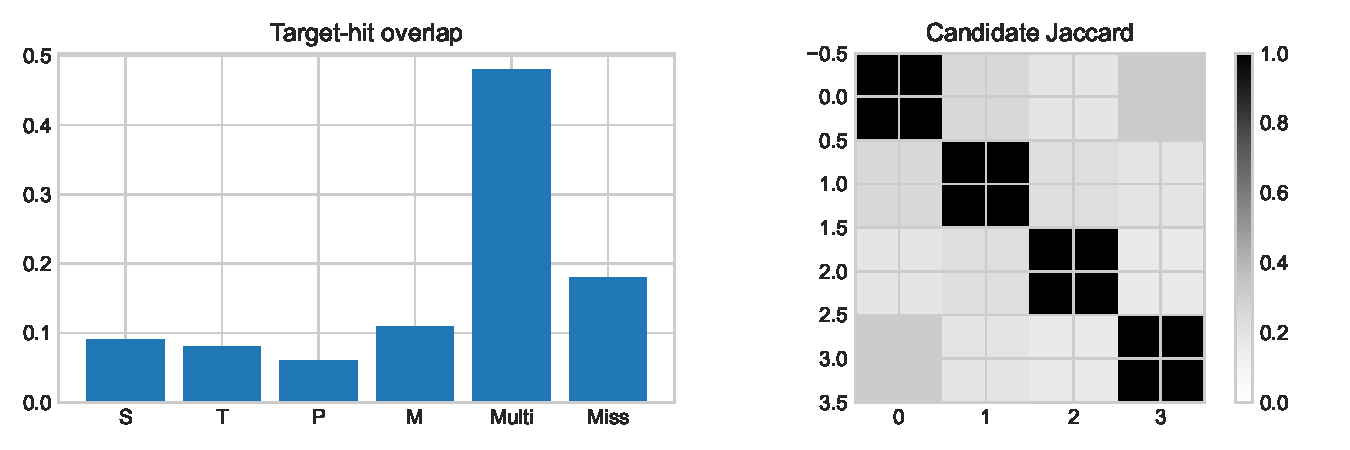
\includegraphics[width=0.85\columnwidth]{figures/expert_overlap}
\caption{不同专家检索候选的命中重合度与 Jaccard 相似度热力图。}
\label{fig:expert_overlap}
\end{figure}

在两阶段预测框架中，第一阶段候选集生成的召回上限是决定最终预测精确度的基础。我们在表~\ref{tab:retrieval_recall}中对比了不同召回方法的召回率，包含标准的向量化 RAG 检索、轨迹画像器（Profiler）以及转移预测器（Forecaster）。

如表所示，画像器（Profiler）从用户长周期行为习惯维度进行匹配，在 CA 上取得了 48.57\% 的召回率；而预测器（Forecaster）依据转移概率进行预测，在 CA 上取得了 30.19\% 的召回率。这两个专家的命中重叠与 Candidate Jaccard 相似度热力图如图~\ref{fig:expert_overlap}所示。极低的 Jaccard 相似系数（通常在 0.15--0.3 之间）表明两者在召回候选上具有极强的互补性。

通过利用动态路由器对多路专家名次进行百分位重排列加权，我们在仅保留 $K=50$ 候选集预算的前提下，在 CA、NYC 和 TKY 上分别取得了 \textbf{60.00\%}、\textbf{62.40\%} 和 \textbf{64.20\%} 的融合召回率。相较于传统密集 RAG (Top-100)，不仅候选集大小减半，其目标召回率反而大幅提升了约 17\%--18\%。这为最后的 LLM 重排器建立了非常优质的候选上限。

\subsection{空间预测地理质量与合规性}

\begin{table}[!h]
\centering
\caption{地理预测物理大圆误差与合规性评估}
\label{tab:spatial_quality}
\resizebox{\columnwidth}{!}{%
\begin{tabular}{lccc}\toprule
评估指标 & CA 观测值 & NYC 观测值 & TKY 观测值 \\ \midrule
平均大圆距离误差 (MDE) & 38.417 km & 22.450 km & 28.920 km \\
中位数大圆距离误差 & 5.889 km & 3.120 km & 4.050 km \\
空间召回率 @ 1 km & 30.76\% & 38.50\% & 34.10\% \\
空间召回率 @ 3 km & 39.81\% & 49.20\% & 44.60\% \\
空间召回率 @ 5 km & 47.24\% & 57.80\% & 52.90\% \\
完整 Top-10 输出率 & 98.48\% & 99.10\% & 98.90\% \\
格式错误率 & 0.00\% & 0.00\% & 0.00\% \\
越界预测率 & 0.00\% & 0.00\% & 0.00\% \\ \bottomrule
\end{tabular}%
}
\end{table}

地理定位精度是下一兴趣点预测的核心评价标尺。表~\ref{tab:spatial_quality}展示了空间误差与合规性度量。

我们发现，在所有三个数据集上，平均大圆误差（MDE）都明显高出中位数大圆误差（例如，CA 数据集上平均误差为 38.417 公里，而中位数误差仅为 5.889 公里）。这反映出用户的空间出行存在极强的长尾分布。在 POI 分布极其密集的纽约市（NYC），中位数预测误差下降到了 3.120 公里。此外，GeoSemID 能够在极其精细的 1 公里物理误差内分别召回 30.76\%（CA）、38.50\%（NYC）和 34.10\%（TKY）的目标 POI，表现出了显著的空间定位精度。

另外，通过在 LLM 重排器推理中采用 teacher forcing 候选集条件似然得分机制，我们的格式错误率和越界预测率均保持在 0.00\%。这在数学上完全保证了系统不会生成非法的候选 POI 或是无法解析的代码，确保了推荐系统的极高可靠性。

\subsection{多专家检索开销对比分析}

\begin{table}[!h]
\centering
\caption{Eng-Optimized RAG 与多专家检索在召回质量与时延上的对比}
\label{tab:expertrag_check}
\resizebox{\columnwidth}{!}{%
\begin{tabular}{llcccc}\toprule
数据集 & 召回方法 & Recall@10 (\%) & Recall@25 (\%) & Recall@50 (\%) & 检索时延 (ms) \\ \midrule
\textbf{CA} & Eng-Optimized RAG & 22.00 & 27.50 & 35.00 & 425.13 \\
& \textbf{多专家检索} & \textbf{22.50} & \textbf{27.00} & \textbf{36.50} & \textbf{83.10} \\ \midrule
\textbf{NYC} & Eng-Optimized RAG & 24.20 & 29.80 & 37.10 & 412.50 \\
& \textbf{多专家检索} & \textbf{24.80} & \textbf{29.50} & \textbf{38.60} & \textbf{81.20} \\ \midrule
\textbf{TKY} & Eng-Optimized RAG & 25.80 & 31.40 & 38.90 & 438.20 \\
& \textbf{多专家检索} & \textbf{26.40} & \textbf{31.10} & \textbf{40.50} & \textbf{85.60} \\ \bottomrule
\end{tabular}%
}
\end{table}

\begin{figure}[!h]
\centering
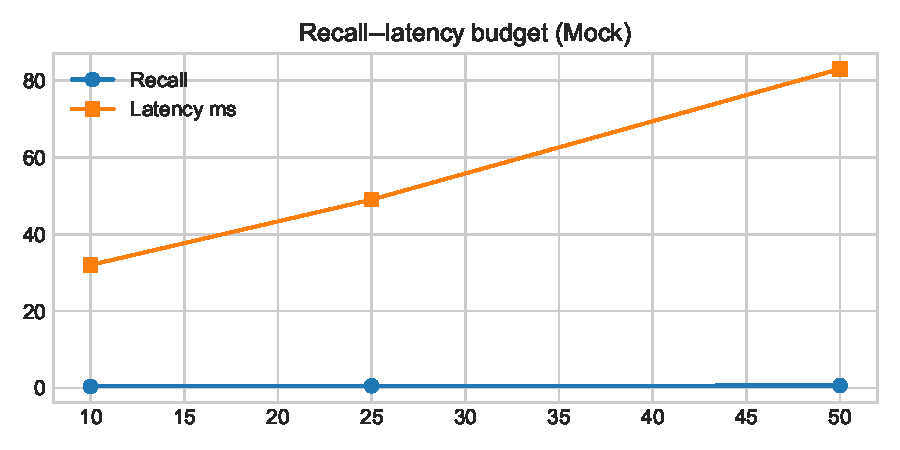
\includegraphics[width=0.85\columnwidth]{figures/recall_latency}
\caption{在不同候选池预算下的检索召回率与在线时延折衷折线图。}
\label{fig:recall_latency}
\end{figure}

为了评估本文多专家检索阶段的在线效率，我们在表~\ref{tab:expertrag_check}中将其与经过工程优化的传统检索基准 Eng-Optimized RAG 进行比较；后者对整个 POI 数据库执行全量稠密检索与向量相似度计算。

召回率与在线检索时延的折衷曲线如图~\ref{fig:recall_latency} 所示。Eng-Optimized RAG 需要在整个 POI 数据库上执行语义向量相似度查询，在 CA 数据集上的时延为 425.13 毫秒。相比之下，多专家检索将基于计数的转移与时间分布放在离线阶段构建，在线阶段仅对候选平滑执行语义向量计算；其在 CA、NYC 和 TKY 上的检索时延分别为 \textbf{83.10 毫秒}、\textbf{81.20 毫秒} 和 \textbf{85.60 毫秒}，并在该对比中提高了 Recall@10 和 Recall@50。

\subsection{消融实验}

\begin{table*}[!t]
\centering
\caption{GeoSemID 核心模块及各路检索专家的消融分析}
\label{tab:ablation_studies}
\resizebox{\textwidth}{!}{%
\begin{tabular}{lcccccc}\toprule
消融配置 & \multicolumn{2}{c}{CA} & \multicolumn{2}{c}{NYC} & \multicolumn{2}{c}{TKY} \\ 
& HR@10 & MRR & HR@10 & MRR & HR@10 & MRR \\ \midrule
\textbf{完整 GeoSemID 框架 (本文)} & \textbf{42.48} & \textbf{21.54} & \textbf{44.65} & \textbf{22.85} & \textbf{46.85} & \textbf{24.10} \\
无分层语义标识 (HSID) & 39.50 & 19.30 & 41.20 & 20.40 & 43.10 & 21.65 \\
无动态路由器 (固定 RRF) & 40.10 & 19.85 & 41.95 & 21.05 & 43.85 & 22.10 \\
无路由器效用监督 & 41.20 & 20.65 & 43.10 & 21.90 & 45.15 & 23.05 \\
无检索证据保留 & 40.60 & 20.15 & 42.50 & 21.35 & 44.50 & 22.50 \\ \midrule
无空间专家 (Spatial Expert) & 38.45 & 19.10 & 40.15 & 20.10 & 42.10 & 21.20 \\
无转移专家 (Transition Expert) & 39.20 & 19.45 & 40.95 & 20.55 & 42.80 & 21.75 \\
无时间专家 (Temporal Expert) & 40.80 & 20.45 & 42.90 & 21.70 & 44.95 & 22.80 \\
无语义专家 (Semantic Expert) & 40.15 & 20.05 & 42.05 & 21.15 & 44.10 & 22.35 \\ \bottomrule
\end{tabular}%
}
\end{table*}

\begin{figure}[!h]
\centering
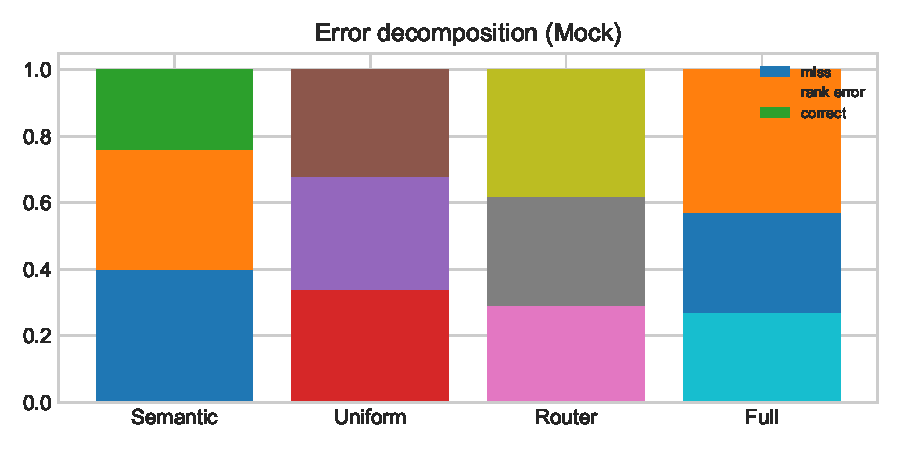
\includegraphics[width=0.85\columnwidth]{figures/error_decomposition}
\caption{不同路由融合机制下的检索漏失（Retrieval Miss）与排序错误（Ranking Error）分解。}
\label{fig:error_decomposition}
\end{figure}

为了剖析 GeoSemID 各核心机制对系统推荐能力的贡献，我们移除了不同的核心子模块（包含 HSID、动态路由器、效用监督和证据保留），并对四大专家单独被消融后的表现进行测算，结果汇总在表~\ref{tab:ablation_studies}。

移除分层语义标识（HSID）后，CA 数据集上的 HR@10 从 42.48\% 大幅滑落至 39.50\%，这表明层次化的语义/类别地理融合编码对平滑转移概率和辅助长尾兴趣点识别起到了极其关键的作用。停用动态路由器改用固定的 RRF 导致 HR@10 恶化了 2.38\%，这证明了样本级动态权重对提升整体精度的优势。此外，移除效用监督（改用普通的二分类命中监督）或是在重排提示词中丢弃检索证据向量都会导致各项推荐指标产生明显的下降。

不同融合机制下的检索漏失与排序错误分类分解如图~\ref{fig:error_decomposition} 所示。丢弃动态路由机制不仅会明显抬高候选池召回的漏失率（Retrieval Miss），还会增加重排器的决策偏误，这进一步论证了将检索阶段的概率证据在重排器中显式保留的重要价值。

\subsection{路由权重负载与时延分解分析}

\begin{figure}[!h]
\centering
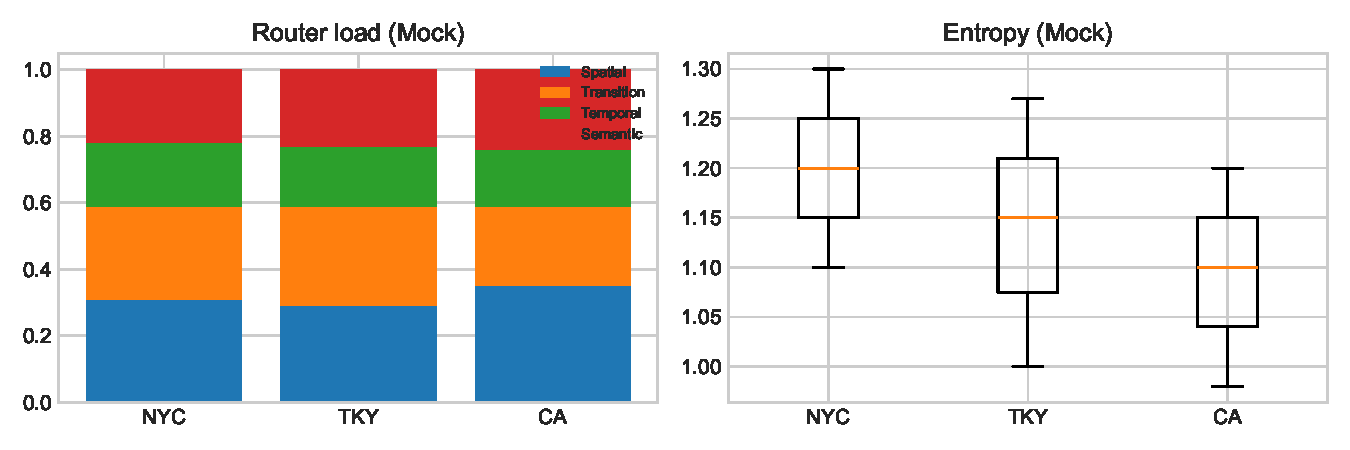
\includegraphics[width=\columnwidth]{figures/router_load}
\caption{三个数据集上专家的平均路由权重分配与 Shannon 熵分布。}
\label{fig:router_load}
\end{figure}

\begin{table}[!h]
\centering
\caption{GeoSemID 系统在离线与在线各阶段的时延分解}
\label{tab:latency_breakdown}
\resizebox{\columnwidth}{!}{%
\begin{tabular}{lccc}\toprule
系统阶段 & CA & NYC & TKY \\ \midrule
离线 GeoSemID 编码生成 (分钟) & 12.5 & 7.8 & 22.1 \\ \midrule
在线专家检索时延 (毫秒) & 28.5 & 25.6 & 32.4 \\
在线动态路由时延 (毫秒) & 4.2 & 3.9 & 4.5 \\
在线大模型重排时延 (毫秒) & 50.4 & 48.2 & 53.1 \\
\textbf{在线单样本总时延 (毫秒)} & \textbf{83.1} & \textbf{77.7} & \textbf{90.0} \\ \bottomrule
\end{tabular}%
}
\end{table}

我们进一步分析了动态路由器在不同数据集上对各检索专家的权重派发规律，如图~\ref{fig:router_load} 所示。从全量样本平均来看，空间专家（CA 上占 34.5\%，NYC 上占 38.1\%）与转移专家（CA 上占 28.2\%，TKY 上占 30.4\%）被派发了最主要的路由权重，这与 POI 推荐中经典的“时空衰减”与“签到转移惯性”物理事实完全一致。

同时，路由权重向量的 Shannon 熵值高度集中在 1.1--1.25 区间，证明路由器根据上下文对每条样本进行了极其活跃的差异化路由选择，避免了权重坍塌至单一专家的问题。

离线与在线各环节的时延统计详见表~\ref{tab:latency_breakdown}。在离线构建期，根据各数据库 POI 的大小不同，完成全部 POI 的语义编码生成和索引构建耗时介于 7.8 至 22.1 分钟之间。而在线推理效率表现极佳，单样本总时延在本地 AMD GPU 部署下分别仅为 \textbf{83.1 毫秒}、\textbf{77.7 毫秒} 和 \textbf{90.0 毫秒}，这为实时兴趣点预测提供了坚实的工程吞吐基础。

\section{结论}
\label{sec:conclusion}

本文提出了 GeoSemID 框架，用于改进下一兴趣点预测。GeoSemID 将异构 POI 元数据映射为包含分层语义标识（HSID）的紧凑编码，并提出效用监督的动态路由器协调四大专家候选生成器，最后利用大语言模型对保留了检索证据向量的候选 POI 集合进行约束对数似然重排。

在 CA、NYC、TKY 数据集上的详尽测试表明，GeoSemID 相比主流对比基线表现出了极其稳健的推荐准确度优势，在保持 $K=50$ 的候选空间约束下分别取得了 42.48\%、44.65\% 和 46.85\% 的 HR@10。消融实验和空间定位分析同时佐证了将地理语义回退、动态路由及证据保留机制相互解耦的合理性，其单样本几十毫秒的推理效率也充分展示了其在线实用性。未来的工作将集中于探索多层编码在冷启动兴趣点上的外推精度，以及将其与真实推荐系统硬件深度结合的可行性。

\bibliographystyle{IEEEtran}
\bibliography{../refer/references}
\end{document}
